\documentclass[UTF8]{ctexart}
\usepackage{bm}
\usepackage{amssymb}
\usepackage{mathtools}
\usepackage{amsmath}
\usepackage{float}
\usepackage{rotating}
\usepackage{booktabs}
\usepackage{pdfpages}

\title{\heiti 最优化第七次作业}
\author{\kaishu 张晋15091060}
\begin{document}
\maketitle
\begin{enumerate}
\item[3.1]
\begin{enumerate}
\item 由题意可列出以下方程:
\begin{align}
&e:\quad x_{eb}=1\\
&b:\quad x_{bc}-x_{eb}=0\\
&d:\quad x_{dc}=5\\
&c:\quad x_{ca}-x_{cd}-x{bc}=-4
\end{align}

解得:
\begin{equation}
x_{eb}=1,x_{bc}=1,x_{ca}=2,x_{cd}=5
\end{equation}

\begin{figure}[H]
\small
\centering
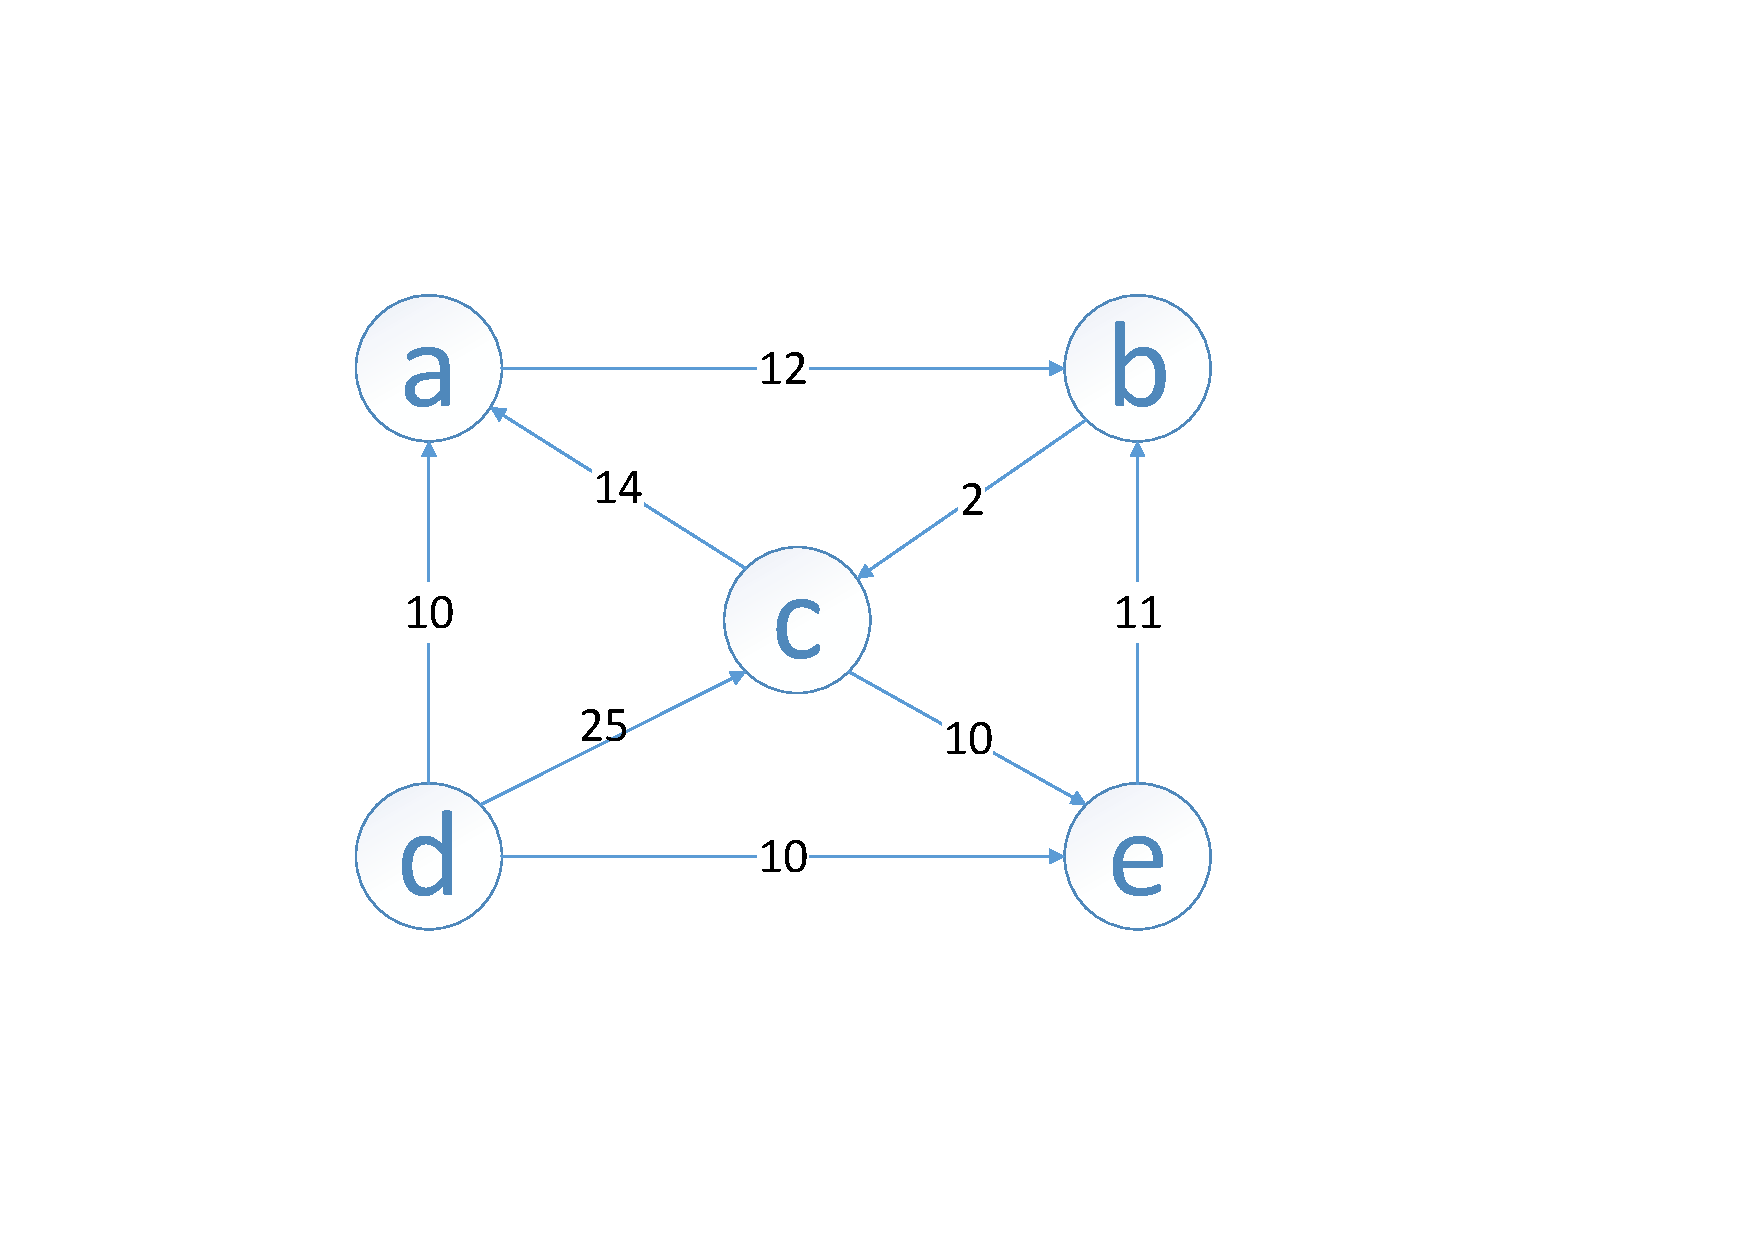
\includegraphics[width=5cm]{1.pdf}
\caption{例图}
\end{figure}

\item 由$y_i-y_j=c_{ij}$得:
\begin{equation}
y_e=0,y_b=-11,y_c=-13,y_a=-27,y_d=12
\end{equation}

\begin{figure}[H]
\small
\centering
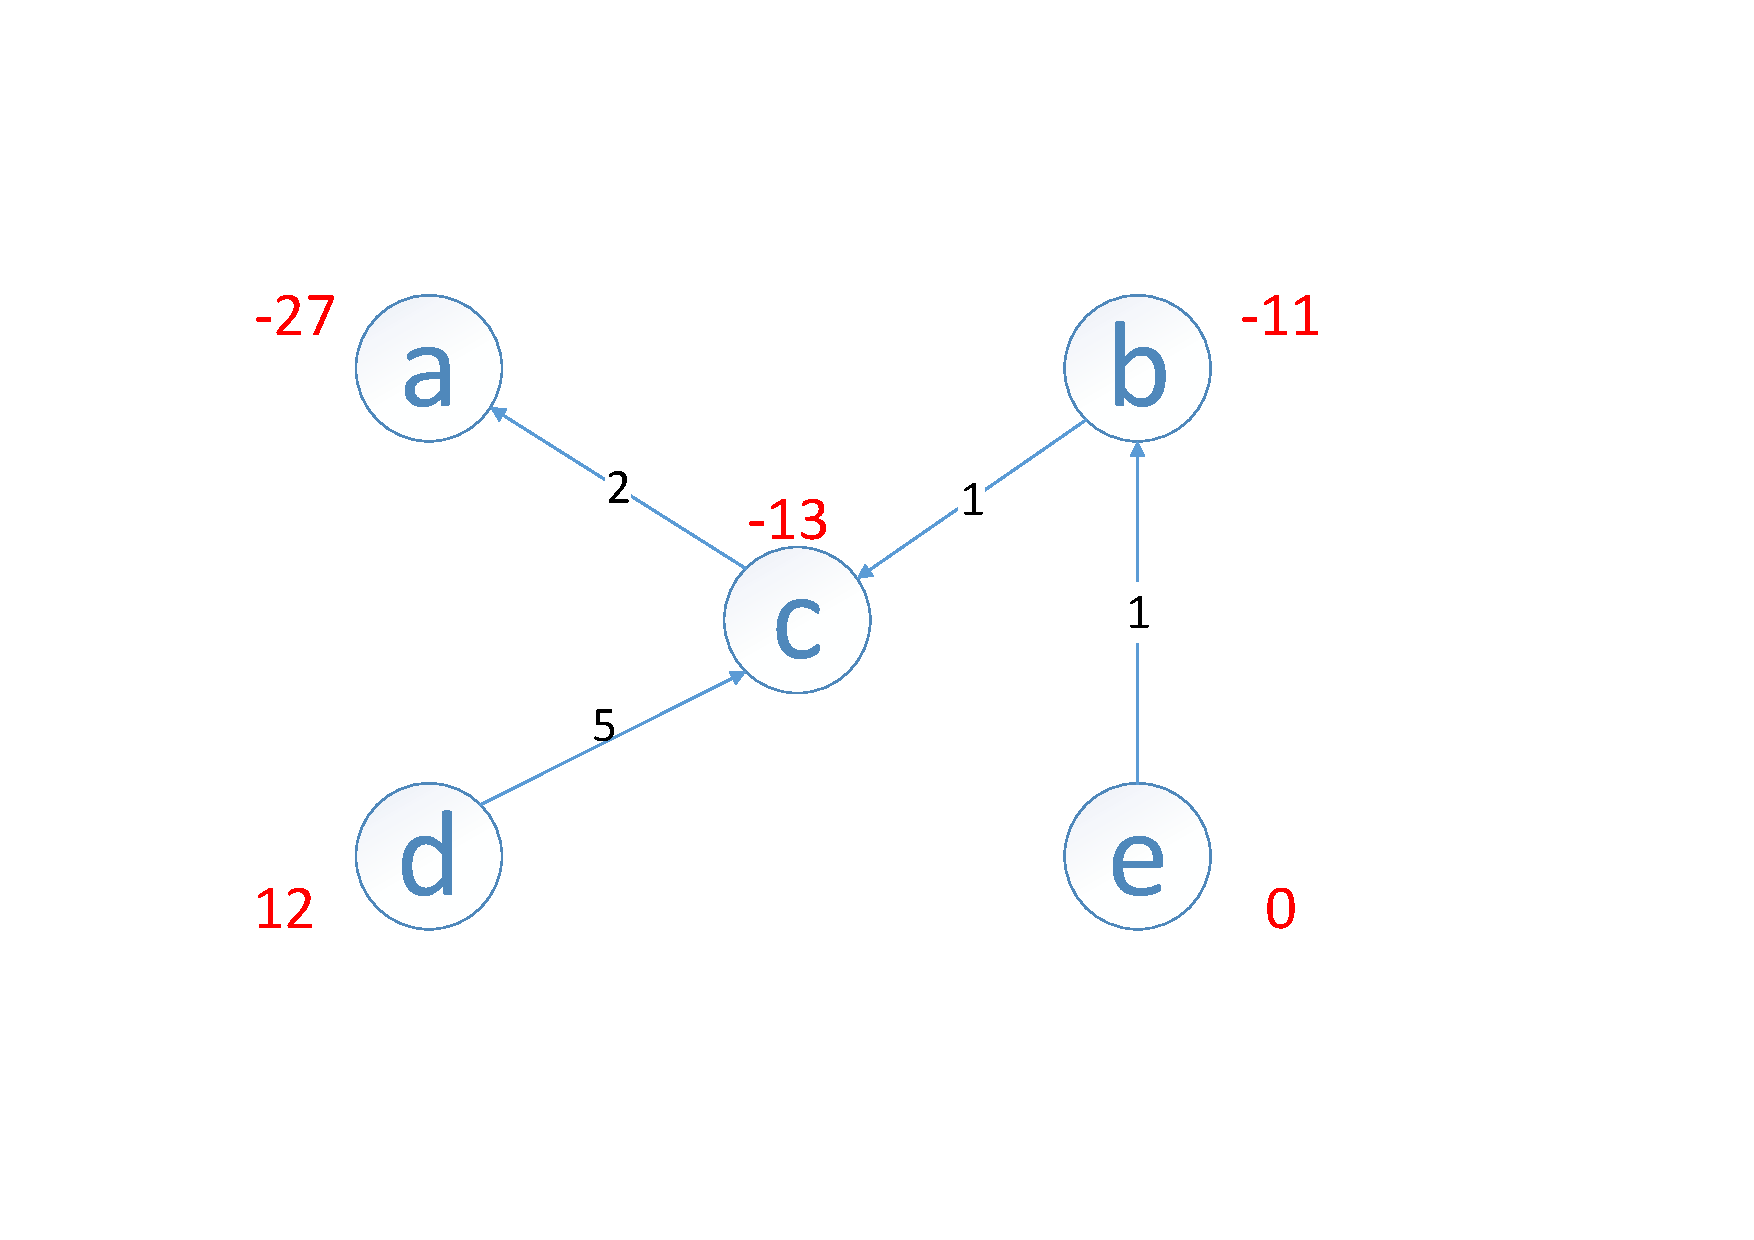
\includegraphics[width=7cm]{2.pdf}
\end{figure}

\item 由$r_{ij}=c_{ij}-(y_i-y_j)$得:
\begin{equation}
r_{ab}=28,r_{ce}=23,r_{de}=-2,r_{da}=-29
\end{equation}
\begin{figure}[H]
\small
\centering
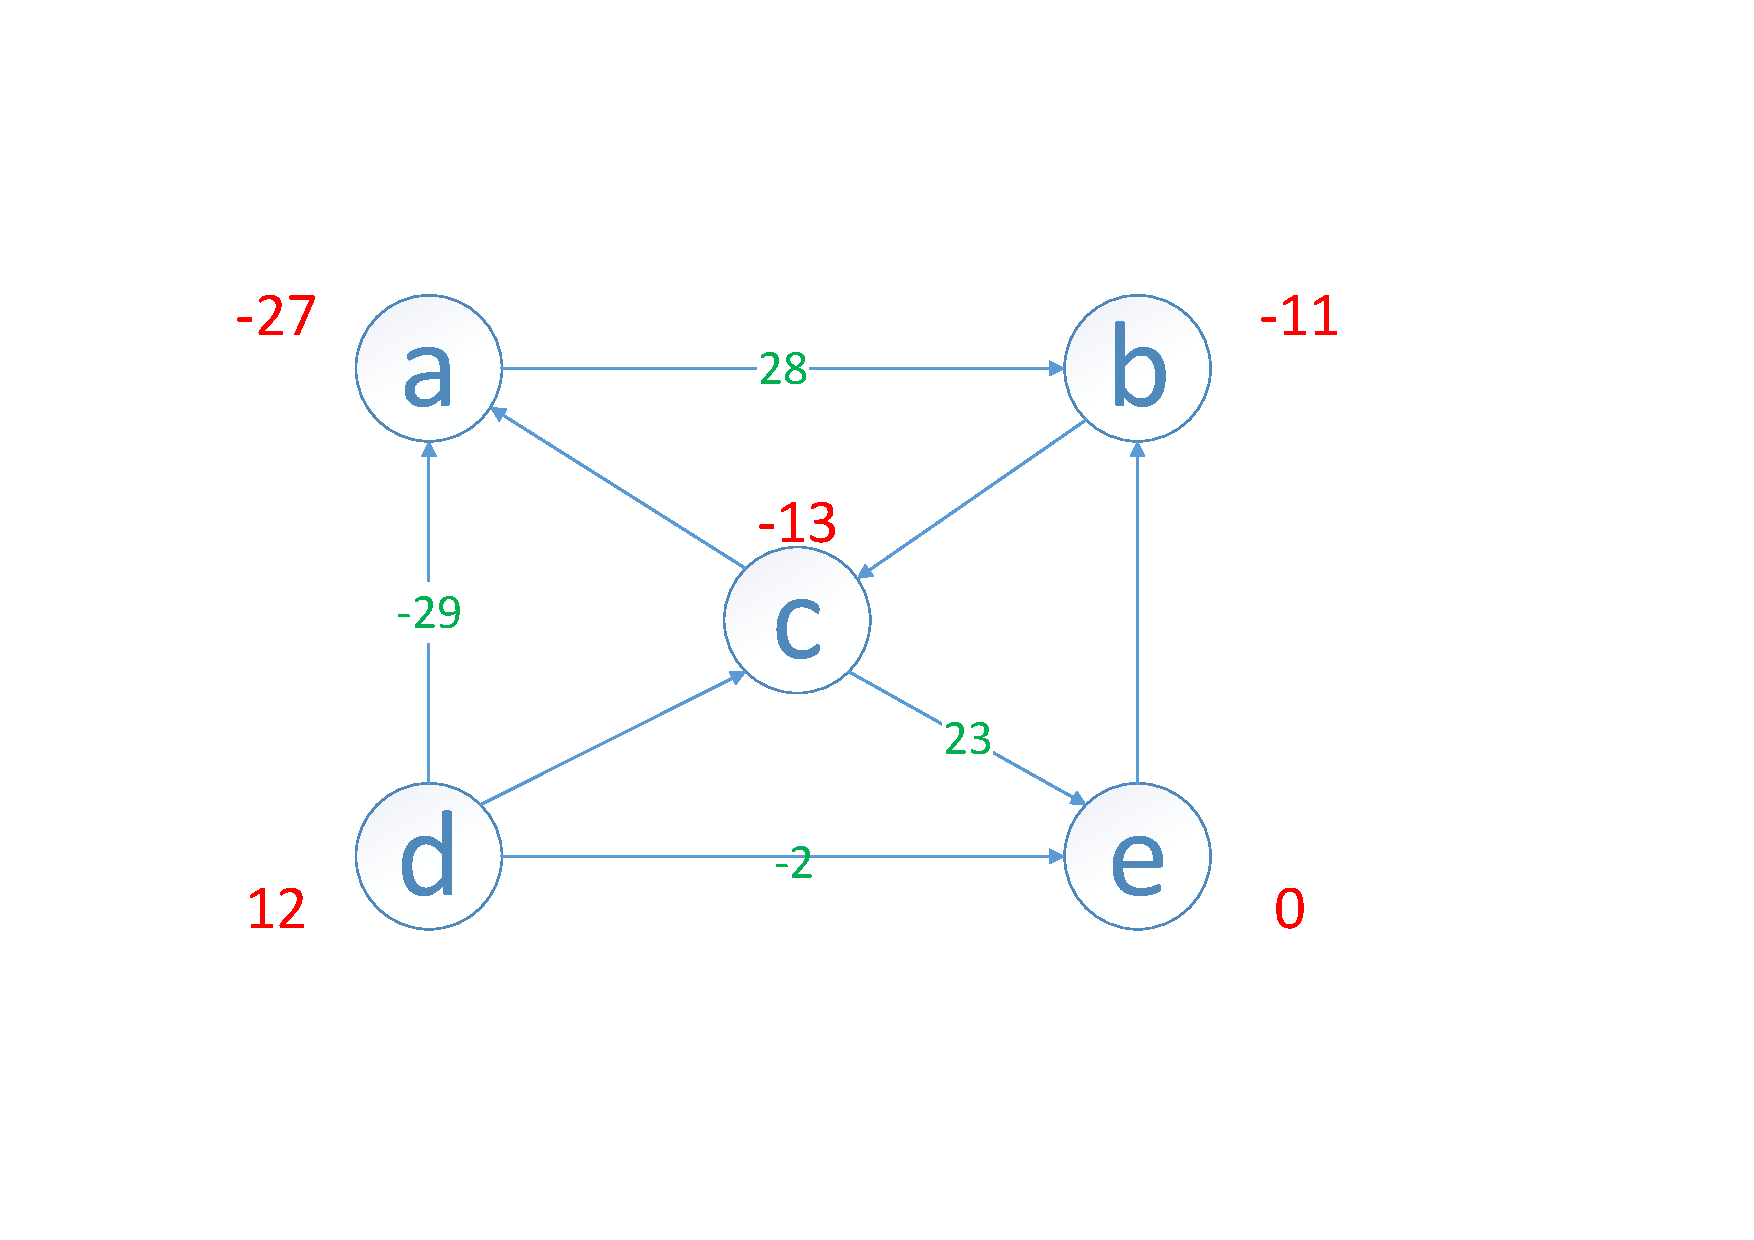
\includegraphics[width=7cm]{3.pdf}
\end{figure}
\end{enumerate}
\item[3.4]
\begin{figure}[H]
\small
\centering
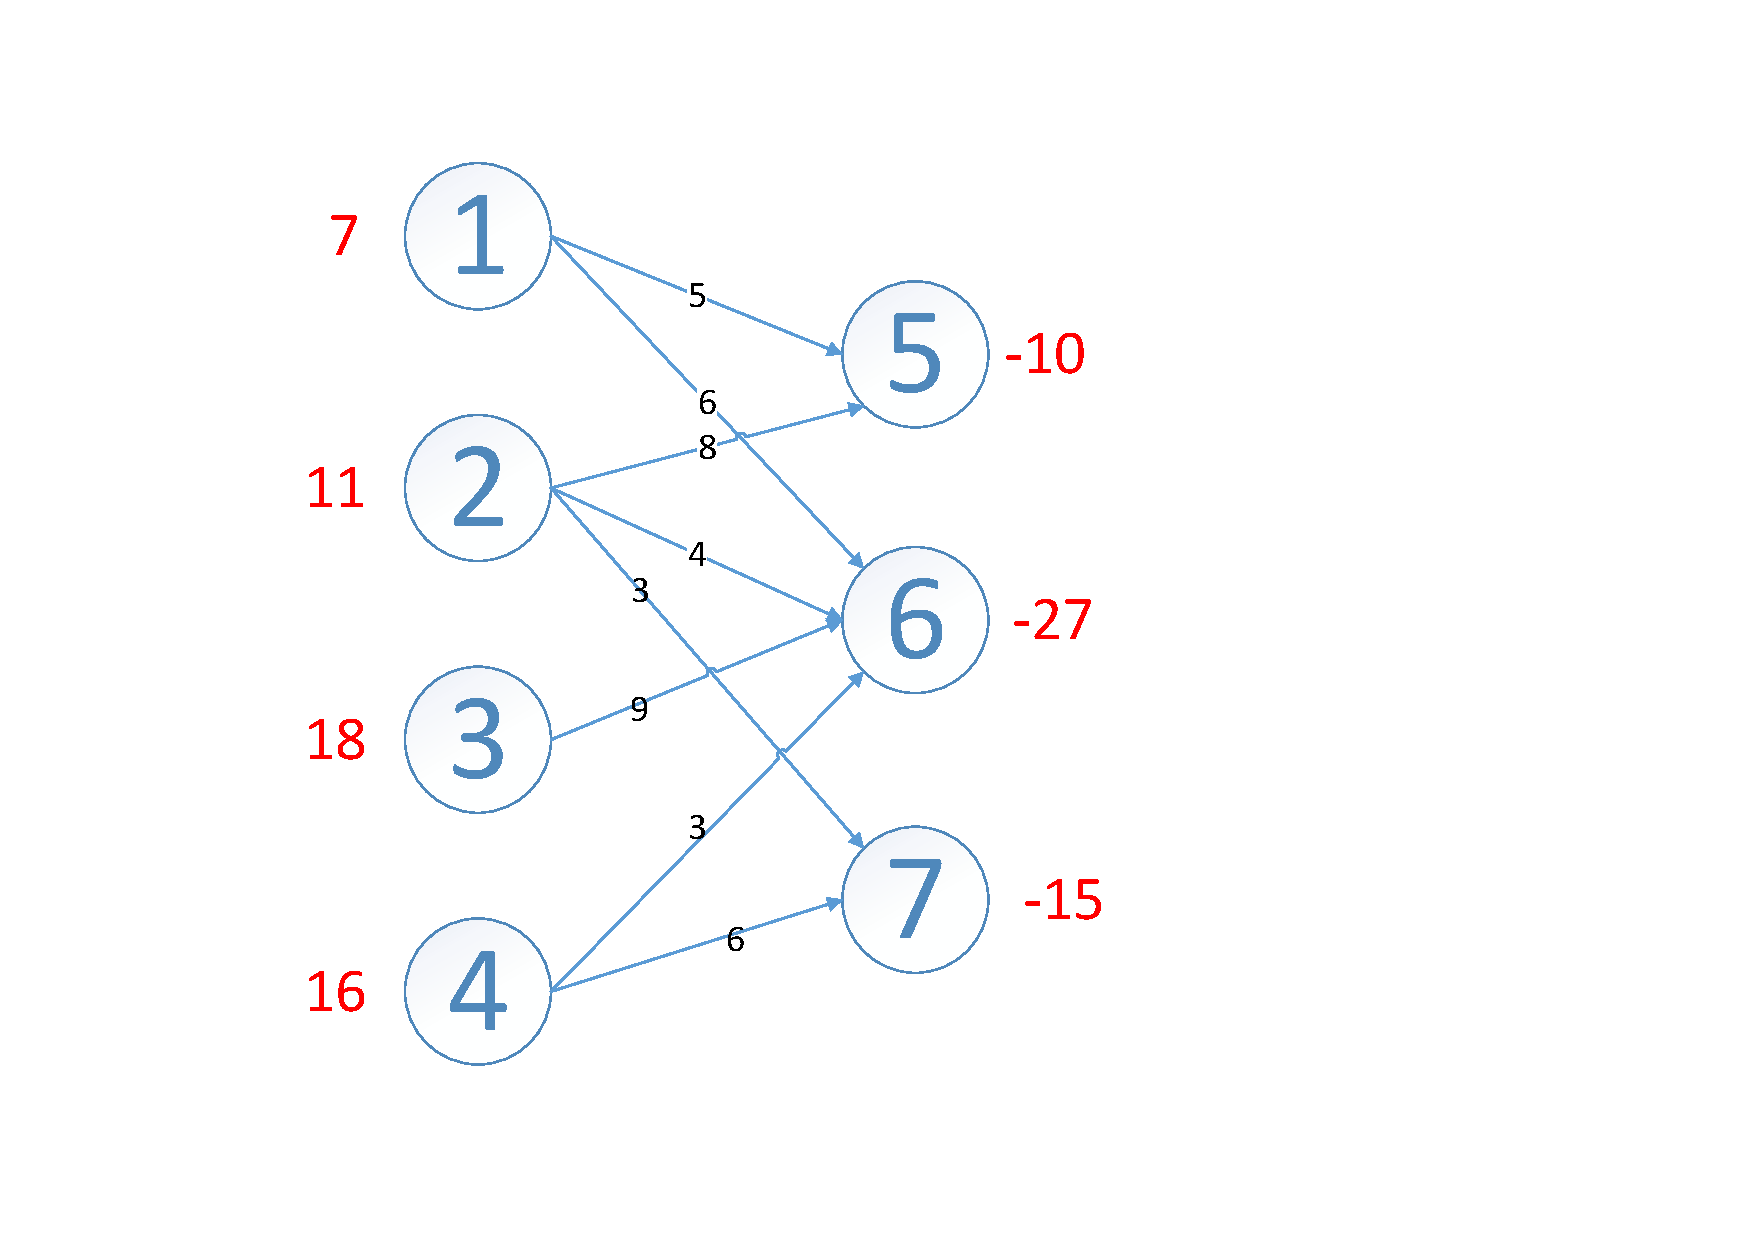
\includegraphics[width=5cm]{4.pdf}
\caption{例图}
\end{figure}
\begin{enumerate}
\item 经计算得:该树解是可行解,但$r_{27}=-8$,因此不是对偶可行的,也不是最优解.


\begin{figure}[H]
\small
\centering
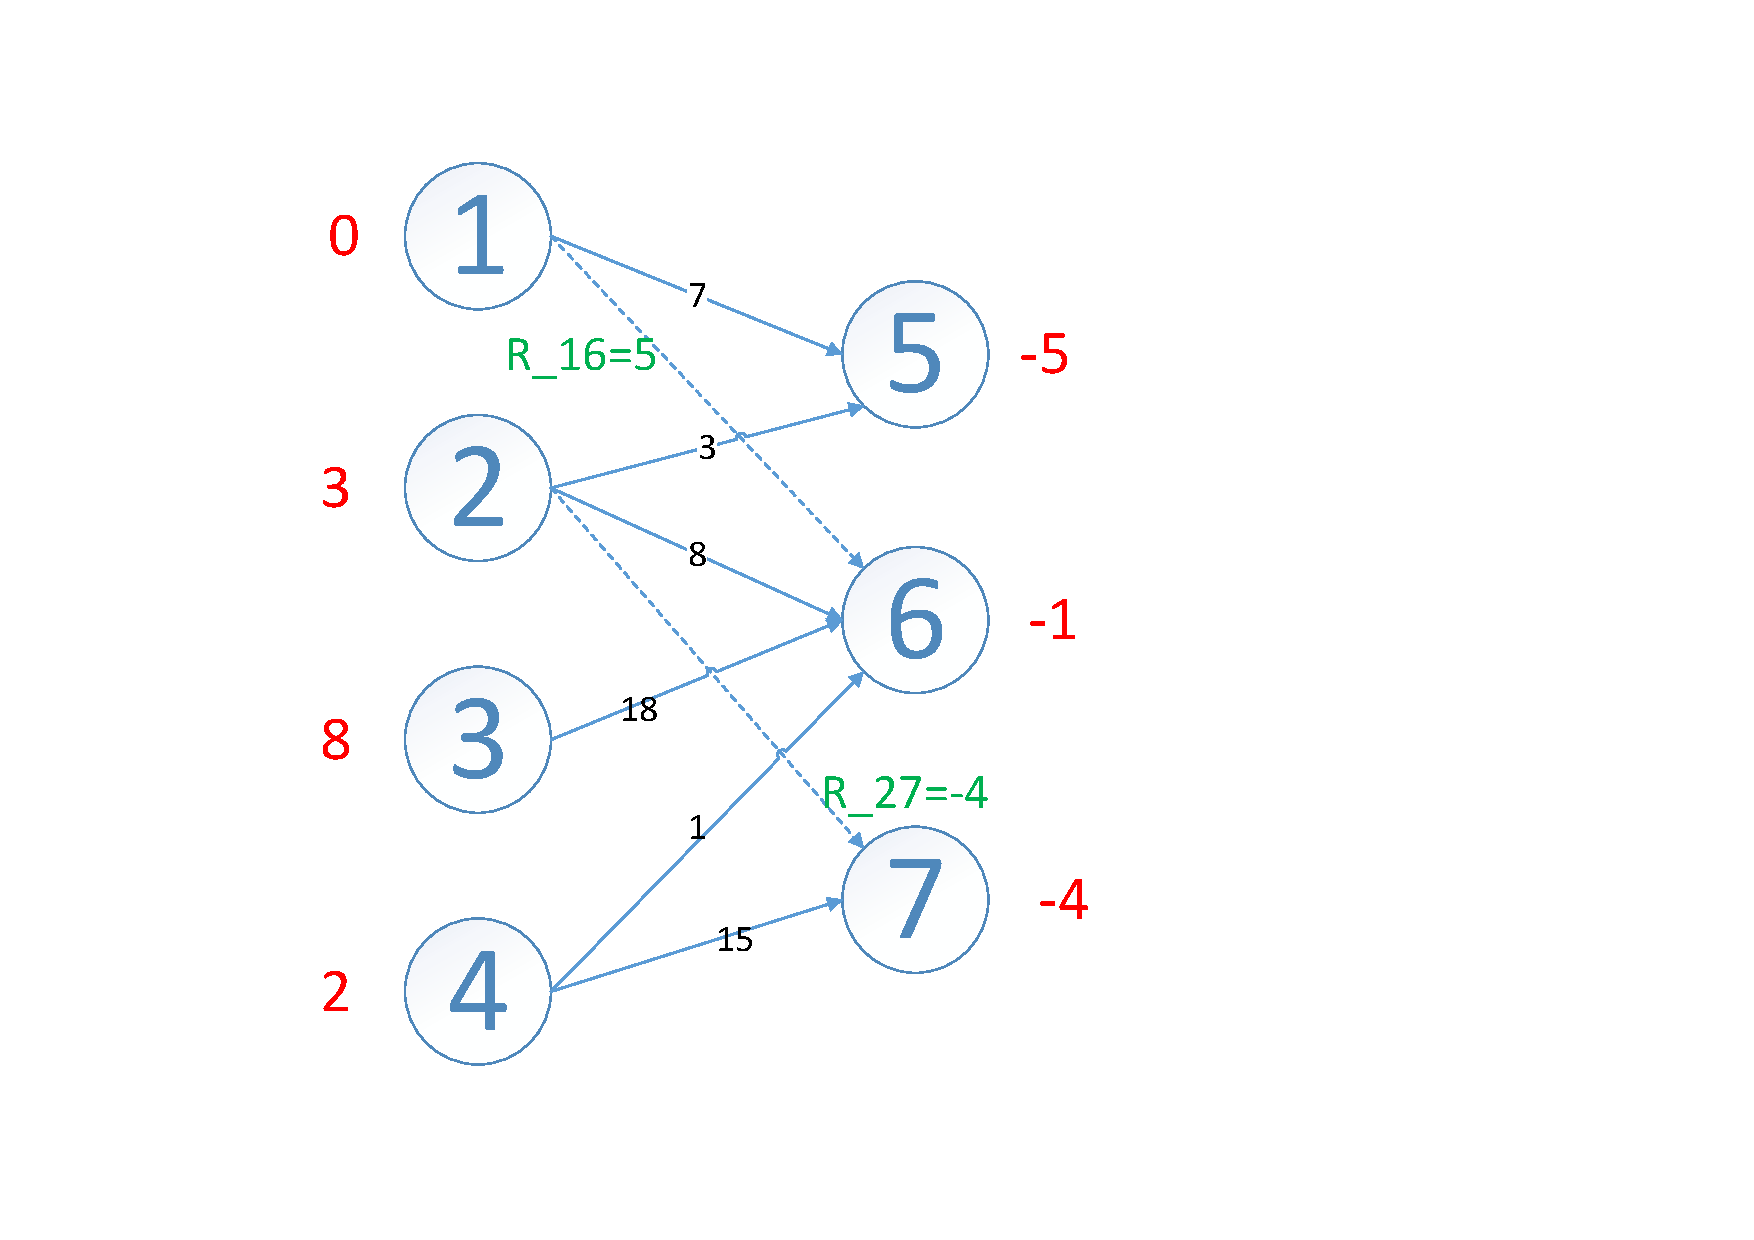
\includegraphics[width=5cm]{5.pdf}
\end{figure}

\item 由于弧$l_{27}$的既约费用系数小于0,首先将弧$l_{27}$进基,然后弧$l_{27},l_{26},l_{46},l_{47}$构成回路,设$l_{27}$上的流量为$t$,当$t$从0逐渐增大时,弧$l_{26}$上的流量先减少到0,故选弧$l_{26}$出基

\begin{figure}[H]
\small
\centering
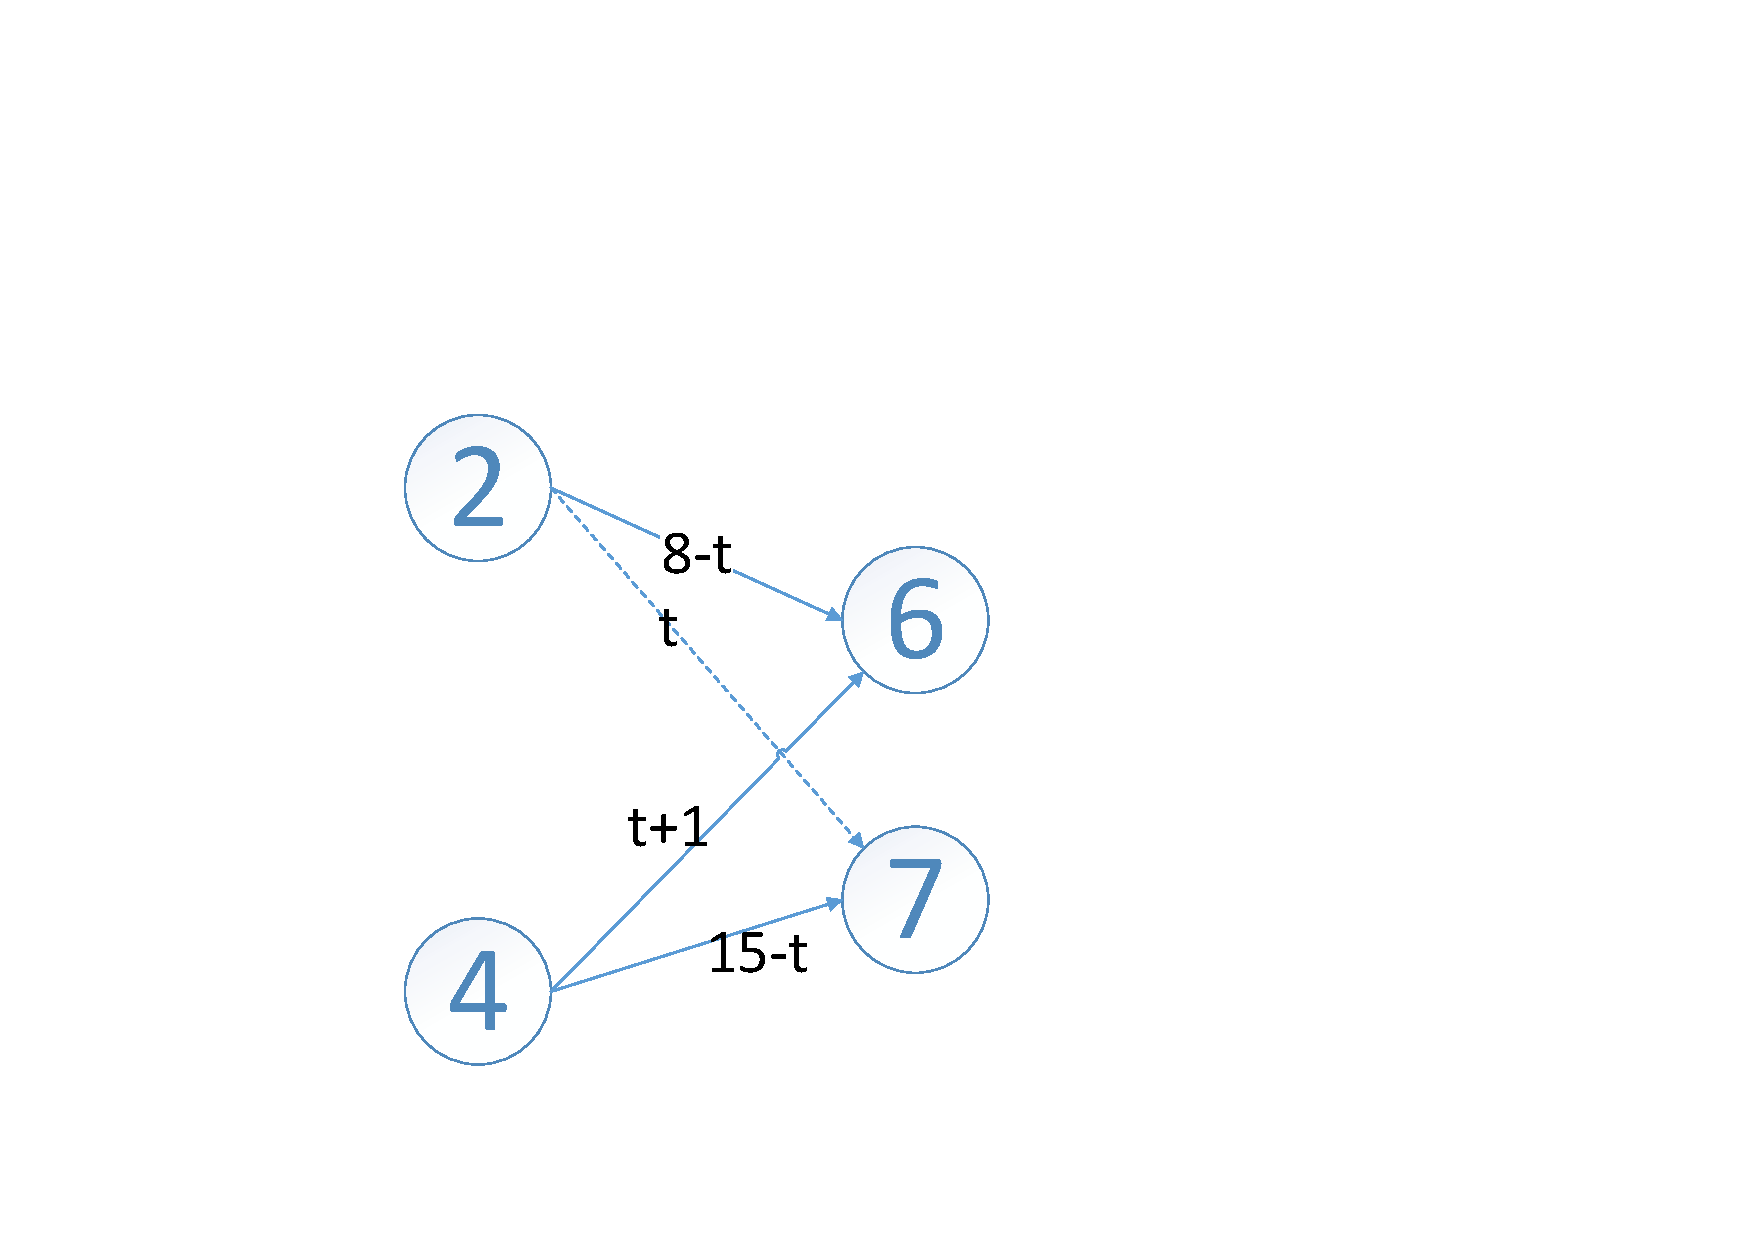
\includegraphics[width=5cm]{6.pdf}
\end{figure}

经计算得,更新后的树解,相对费用系数都大于0,所得即为最优解,最小费用为314,每条边的流量如图3所示.

\begin{figure}[H]
\small
\centering
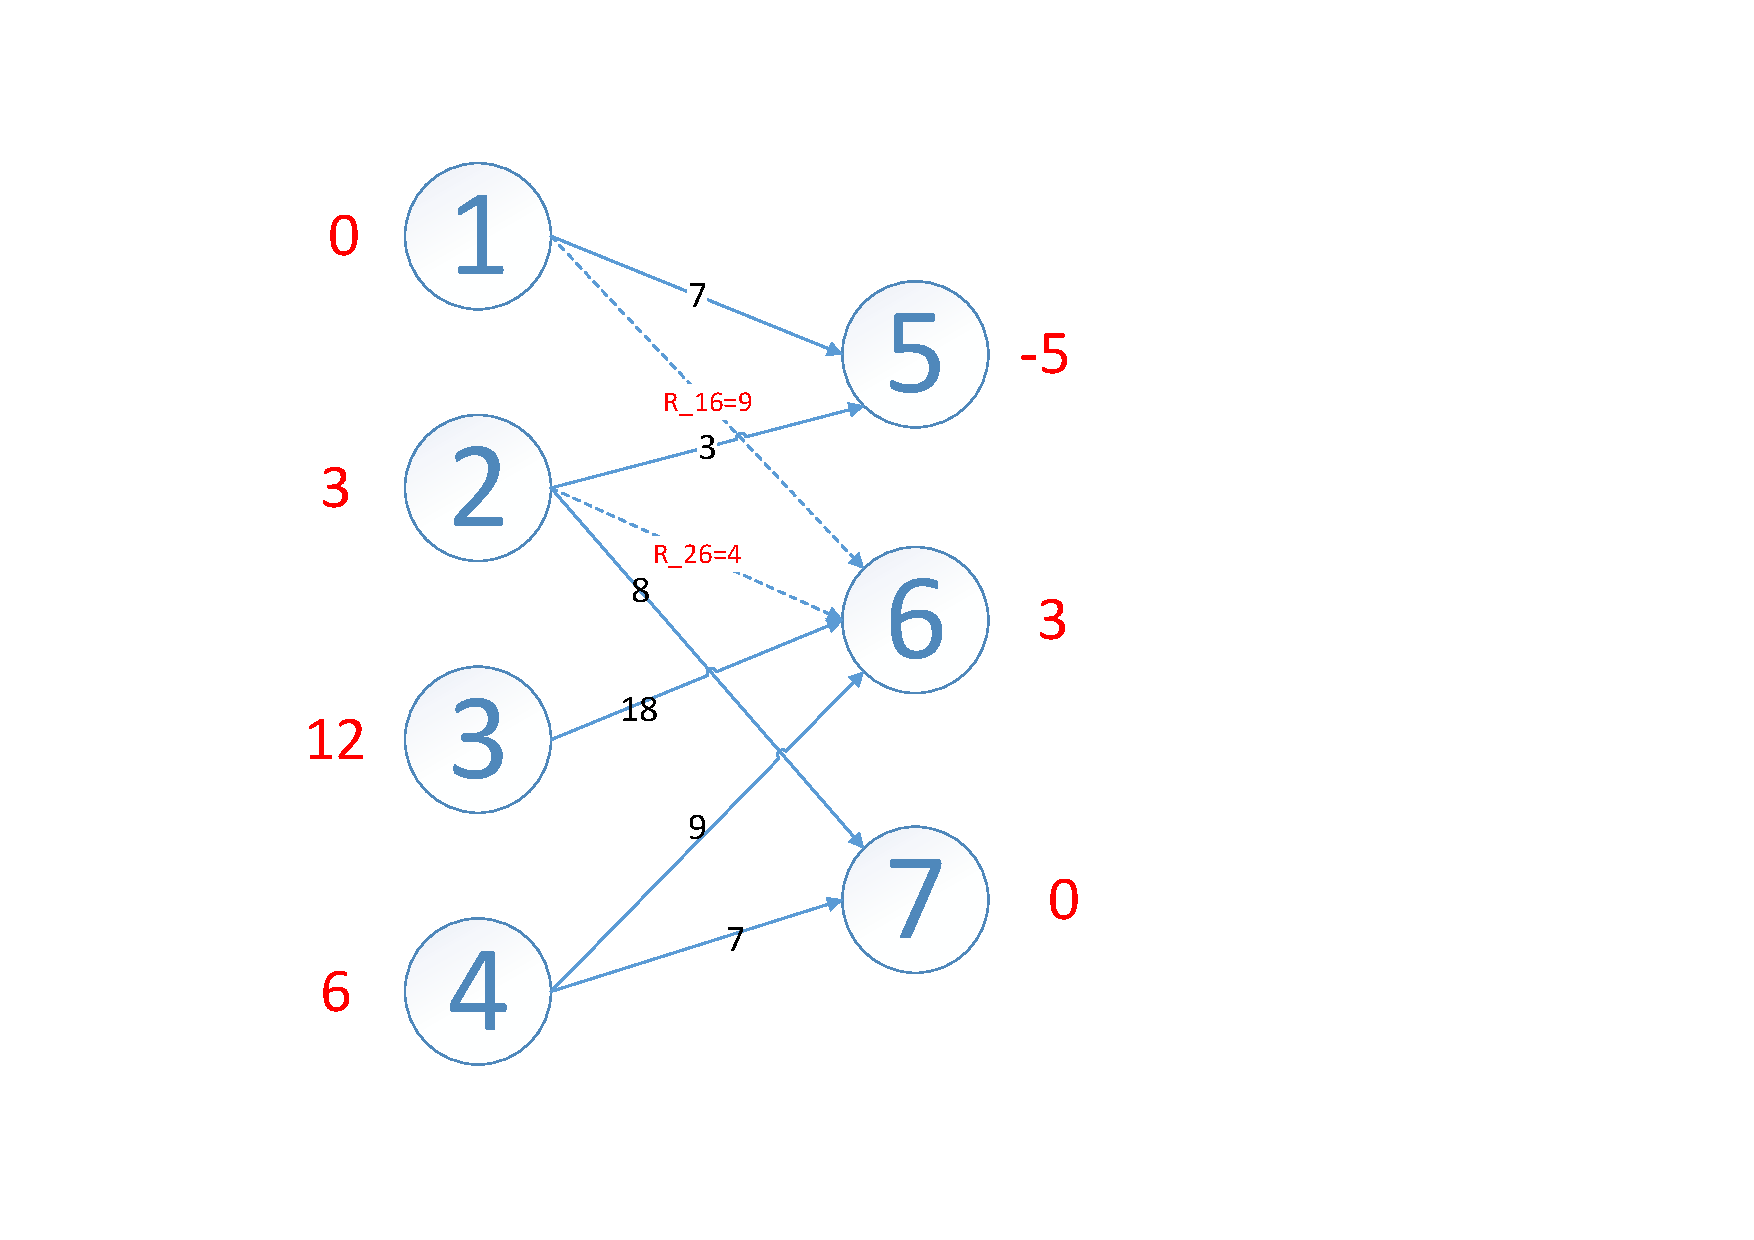
\includegraphics[width=8cm]{9.pdf}
\caption{最优树解}
\end{figure}
\end{enumerate}
\end{enumerate}


\end{document}